\todo{Wichtige Begriffe erklären}
\subsection{Element- und Verbindungshalbleiter}
	\subsubsection{Direkte und indirekte Halbleiter}
	Direkte und indirekte Halbleiter unterscheiden sich in der Position des Minimums / Maximums im Bänderdiagramm .......
	
		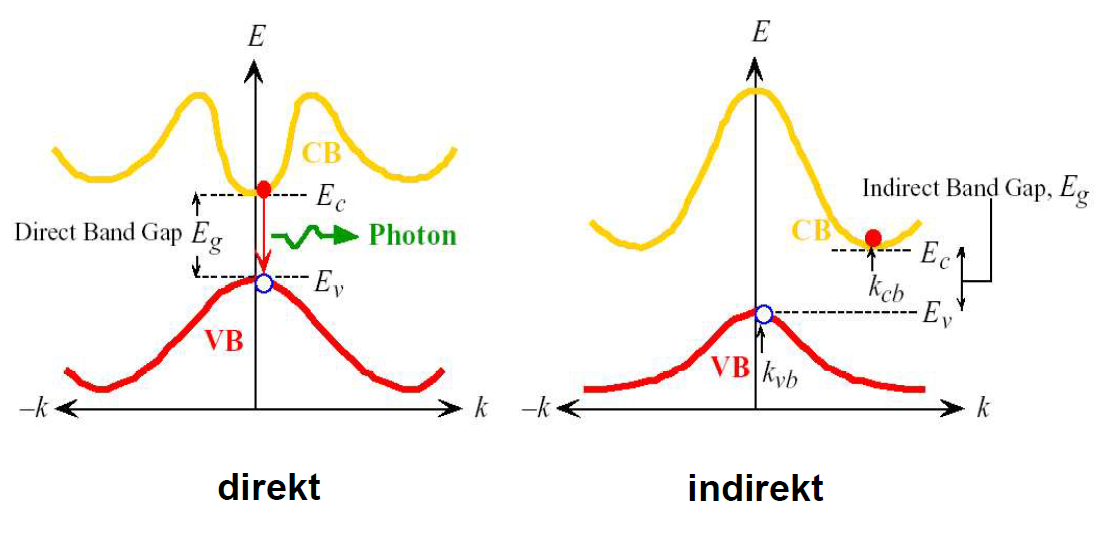
\includegraphics[width=\linewidth]{Kapitel/Kap11/direkte_indirekte_halbleiter.PNG}
	
	\subsubsection{Dotieren von Verbindungshalbleitern}
	
	 Bla Bla Bla
	\subsubsection{Ladungsträgerbeweglichkeiten}
\subsection{Welleneigenschaften}
	\subsubsection{Monochromatisch} 
	\subsubsection{kohärent} \subsubsection{kollimiert}
\subsection{Leuchtdioden}
	\subsubsection{Funktionsprinzip}
	\subsubsection{Verschiedene Farben}
	\subsubsection{Weiße Dioden}
\subsection{Laser}
	\subsubsection{Funktionsprinzip (stimulierte Emission, Pumpen, beteiligte Energieniveaus, ...)}
	
	\subsubsection{Resonatoren}
	\subsubsection{Halbleiterlaser (Prinzipeller Aufbau, VCSEL, ...)}


\todo{Fragen aus Own Clowd zuordnen}
\todo{Gruppenübungs-Inhalte ergänzen}